\documentclass[a4paper,12pt]{article} 

\usepackage[top = 2.5cm, bottom = 2.5cm, left = 2.5cm, right = 2.5cm]{geometry} 

\usepackage[T1]{fontenc}
\usepackage[utf8]{inputenc}
\usepackage{amsmath}
\usepackage{multirow}
\usepackage{booktabs} 
\usepackage{tikz}
\usepackage{float,graphicx} 
\usepackage{amssymb} 
\usepackage{pdfpages}
\usepackage{adjustbox}
\usepackage{setspace}
\setlength{\parindent}{0in}

\usepackage{float}

\usepackage{fancyhdr}
\usepackage{enumerate}


\pagestyle{fancy} 
\fancyhf{}
\lhead{\footnotesize PR \& ML: Blatt 4}
\rhead{\footnotesize F. Freter, E. Kirchberger, S. Symhoven \& J. Wustl} %<---- Fill in your lastnames.

\cfoot{\footnotesize \thepage} 

\begin{document}

\thispagestyle{empty} 

\begin{tabular}{p{15.5cm}} 
{\large \bf Pattern Recognition und Machine Learning} \\
Hochschule München \\ Sommersemester 2023  \\ Prof. Dr.-Ing. Claudius Schnörr \\
\hline 
\\
\end{tabular} 

\vspace*{0.3cm} 

\begin{center} 
	{\Large \bf Blatt 4} 
	\vspace{2mm}
	

	{\bf F. Freter, E. Kirchberger, S. Symhoven \& J. Wustl} 
		
\end{center}  

\vspace{0.4cm}

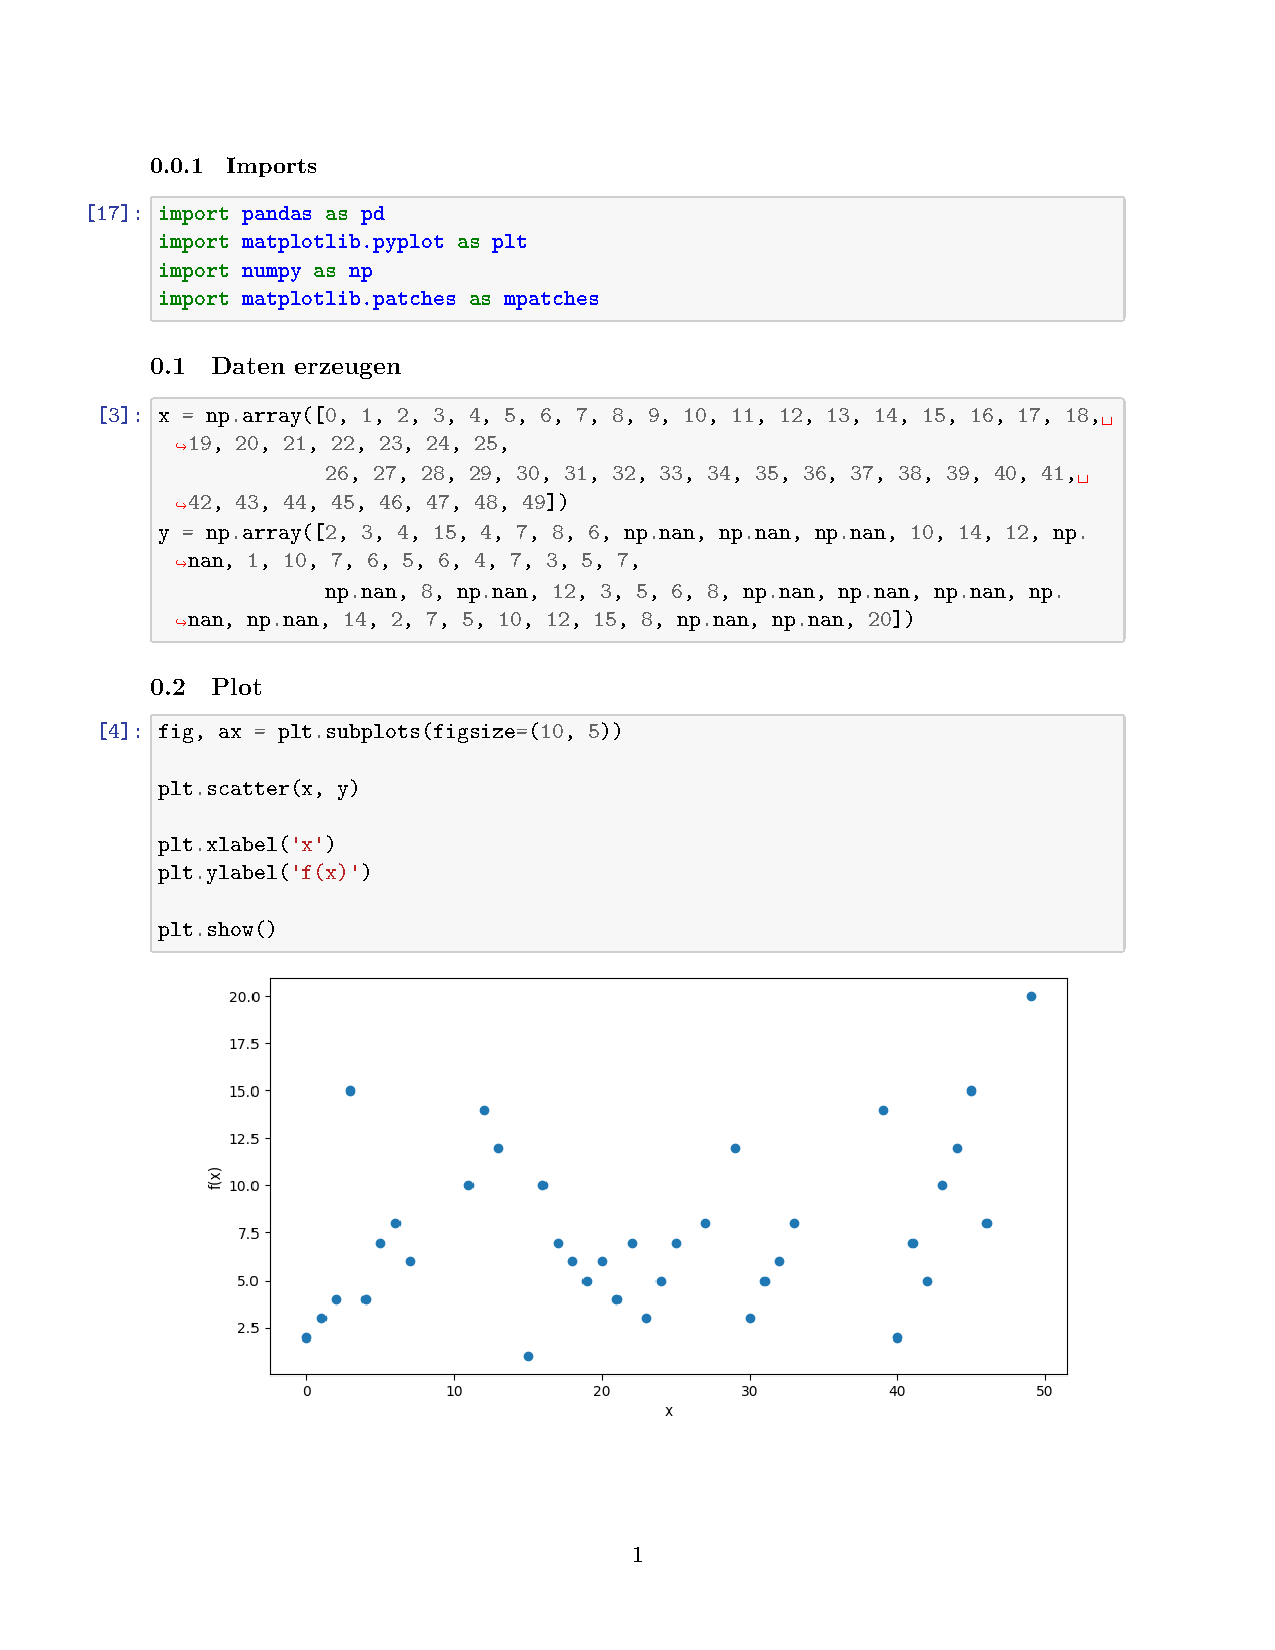
\includepdf[pages=1,pagecommand=\section*{Aufgabe 1/2: Lineare Regression}]{aufgabe-1-2.pdf}
\includepdf[pages={2-}]{aufgabe-1-2.pdf}

\section*{Aufgabe 3: Support Vektor Maschinen}

\subsection*{SVM-Klassifikation:}

\begin{enumerate}

	\item Aufgabe 1 
	
	\item
		\begin{figure}[H]
			\centering
			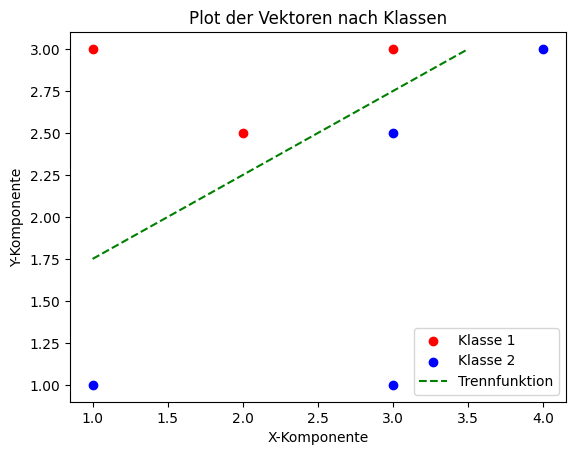
\includegraphics[width = .7\linewidth]{aufgabe-4-2.png}
	  	\end{figure}

		Ja, es handelt sich dabei um eine linear trennbare Problemstellung. Diese kann über zwei Punkte 
		$a=\begin{pmatrix} 1 \\ 1.75 \end{pmatrix}$ und $b=\begin{pmatrix} 3.5 \\ 3 \end{pmatrix}$ definiert werden 
		und maximiert den Rand zwsichen den beiden Klassen:

		\[f_f(x)=0.5x+1.25\]
	

	\item
	
	\item
	
	\item
	
	\item
	
	\item


\end{enumerate}


\subsection*{SVM-Regression:}

\end{document}
